\documentclass[11pt]{article}
\usepackage{geometry}
\geometry{margin=1in}
\usepackage{amssymb}
\usepackage{enumitem}
\usepackage{parskip}
\usepackage{xcolor}
\usepackage{tikz}
\definecolor{benblue}{HTML}{1769AA}
\definecolor{benorange}{HTML}{C2410C}

\newcommand{\drawbox}[1]{%
  \par\vspace{4pt}\noindent
  \fbox{\rule{0pt}{#1}\rule{\dimexpr\linewidth-2\fboxsep-2\fboxrule}{0pt}}%
  \par\vspace{6pt}}

\newcommand{\task}[1]{\par\medskip\noindent\textbf{\color{benblue}#1}\par\nopagebreak}

\title{\vspace{-1.5cm}\textbf{Pythagoras}\\[-2pt]
  \large Proofs you can see}
\author{}
\date{}

\begin{document}
\maketitle
\vspace{-1.2cm}

\noindent\textbf{The setup.} A \emph{right triangle} has one 90-degree corner.
The two short sides touching it are the \emph{legs}, $a$ and $b$. The long side
across from it is the \emph{hypotenuse}, $c$. The claim:
\[ a^2 + b^2 = c^2. \]
We are not going to memorize it. We are going to \emph{see} why it must be true.

\section*{Build 1: three squares on a 3-4-5 triangle}
On grid paper, draw a right triangle with legs $3$ and $4$. On each side, draw the
square that sticks out away from the triangle (like the picture). Count the boxes
in each square.

\begin{center}
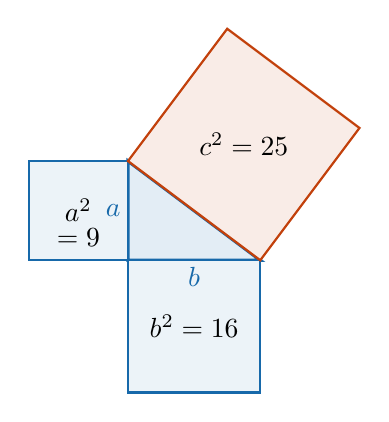
\begin{tikzpicture}[scale=0.42]
  % triangle
  \fill[benblue!12] (0,0) -- (4,0) -- (0,3) -- cycle;
  \draw[benblue, very thick] (0,0) -- (4,0) -- (0,3) -- cycle;
  % square on leg b=4 (downward)
  \draw[benblue, thick, fill=benblue!8] (0,0) -- (4,0) -- (4,-4) -- (0,-4) -- cycle;
  \node at (2,-2) {$b^2=16$};
  % square on leg a=3 (leftward)
  \draw[benblue, thick, fill=benblue!8] (0,0) -- (0,3) -- (-3,3) -- (-3,0) -- cycle;
  \node at (-1.5,1.5) {$a^2$};
  \node at (-1.5,0.7) {$=9$};
  % square on hypotenuse (outward), normal (3,4)
  \draw[benorange, thick, fill=benorange!10]
        (4,0) -- (0,3) -- (3,7) -- (7,4) -- cycle;
  \node at (3.5,3.5) {$c^2=25$};
  \node[benblue] at (-0.45,1.5) {$a$};
  \node[benblue] at (2,-0.5) {$b$};
\end{tikzpicture}
\end{center}

\task{Add the two leg squares: $9 + 16 = $ \underline{\hspace{1.6cm}}. Now look at
the big tilted square. What is its area? \underline{\hspace{1.6cm}}}

\task{Draw your own version on grid paper here:}
\drawbox{1.4cm}

\section*{Build 2: count a tilted square}
You cannot read off the side of a tilted square, so use this trick. Box the tilted
square inside the smallest \emph{upright} square (for 3-4-5 it is a $7\times 7$
box, area $49$). Four copies of your triangle sit in the corners, each of area
$\frac{1}{2}(3)(4) = 6$.

\task{Tilted square area $= 49 - 4\times 6 = $ \underline{\hspace{1.6cm}}.
Does it match Build 1? \underline{\hspace{1.6cm}}}

\section*{See the proof: the tilted square}
A big square of side $a+b$ holds four copies of the triangle, leaving a tilted
square of side $c$ in the middle.

\begin{center}
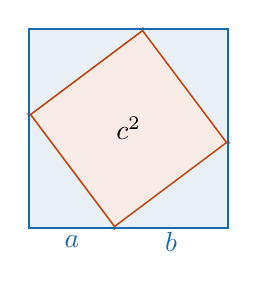
\begin{tikzpicture}[scale=0.36]
  % outer square side 7
  \draw[gray, thick] (0,0) rectangle (7,7);
  % inner tilted square: (3,0),(7,3),(4,7),(0,4)
  \draw[benorange, very thick, fill=benorange!10]
        (3,0) -- (7,3) -- (4,7) -- (0,4) -- cycle;
  \node at (3.5,3.5) {$c^2$};
  % four corner triangles shaded lightly
  \fill[benblue!10] (3,0) -- (7,0) -- (7,3) -- cycle;
  \fill[benblue!10] (7,3) -- (7,7) -- (4,7) -- cycle;
  \fill[benblue!10] (4,7) -- (0,7) -- (0,4) -- cycle;
  \fill[benblue!10] (0,4) -- (0,0) -- (3,0) -- cycle;
  \draw[benblue, thick] (3,0) -- (7,0) -- (7,3);
  \draw[benblue, thick] (7,3) -- (7,7) -- (4,7);
  \draw[benblue, thick] (4,7) -- (0,7) -- (0,4);
  \draw[benblue, thick] (0,4) -- (0,0) -- (3,0);
  \node[benblue] at (1.5,-0.5) {$a$};
  \node[benblue] at (5,-0.5) {$b$};
\end{tikzpicture}
\end{center}

\task{Find the big square's area two ways, then set them equal.}
\begin{itemize}[leftmargin=*]
  \item As one square: $(a+b)^2 = $ \underline{\hspace{4.5cm}}
  \item As pieces: four triangles $+$ the hole $= $ \underline{\hspace{3.6cm}}
\end{itemize}
\task{Set them equal, cancel the $2ab$, and write what is left:}
\drawbox{1.3cm}

\section*{Push further}
\begin{enumerate}[leftmargin=*]
  \item \textbf{The triple machine.} Pick whole numbers $m > n$. Then
        $\big(m^2 - n^2,\ 2mn,\ m^2 + n^2\big)$ is always a Pythagorean triple.
        Fill the table and check each one squares correctly.

        \medskip
        \begin{center}
        \begin{tabular}{c c | c c c | c}
          $m$ & $n$ & $m^2-n^2$ & $2mn$ & $m^2+n^2$ & check \\ \hline
          $2$ & $1$ & \rule{1.4cm}{0pt} & \rule{1.4cm}{0pt} & \rule{1.4cm}{0pt} & \rule{2.4cm}{0pt}\\[7pt]
          $3$ & $2$ & & & & \\[7pt]
          $4$ & $1$ & & & & \\[7pt]
          $4$ & $3$ & & & & \\[7pt]
        \end{tabular}
        \end{center}

  \item \textbf{Competition gem (the converse).} The theorem says: right angle
        $\Rightarrow a^2+b^2=c^2$. The converse runs the arrow the other way: if
        $a^2+b^2=c^2$, the angle opposite $c$ \emph{must} be a right angle. This
        is why a knotted 3-4-5 rope makes a perfect right corner. Prove it. (Hint:
        build a brand-new right triangle with legs $a$ and $b$. What is its
        hypotenuse, and how does that pin down your triangle's angle?)
        \drawbox{1.7cm}

  \item \textbf{True or false?} Guess first, then ask.
        \begin{itemize}
          \item $a^2+b^2=c^2$ works for \emph{any} triangle, not just right ones.
                \hfill T \quad / \quad F
          \item A box with edges $a,b,c$ has space diagonal $d$ with
                $d^2=a^2+b^2+c^2$. \hfill T \quad / \quad F
          \item There are only finitely many Pythagorean triples.
                \hfill T \quad / \quad F
        \end{itemize}
\end{enumerate}

\end{document}
